% The side predicates: how side1 to side4 are derived, and how they are evaluated.
%
% A companion to ../../design_document/DESIGN.tex (section 6) and to
% code/src/kernel/side.h. Build with
%
%   latexmk -pdf side_predicates.tex        or        pdflatex side_predicates.tex (twice)
\documentclass[11pt,a4paper]{article}

\usepackage[T1]{fontenc}
\usepackage[utf8]{inputenc}
\usepackage{lmodern}
\usepackage[british]{babel}
\usepackage[a4paper,margin=2.5cm]{geometry}
\usepackage{microtype}
\usepackage{amsmath,amssymb,amsthm,mathtools}
\usepackage{array,booktabs,tabularx}
\usepackage[shortlabels]{enumitem}
\usepackage{xcolor}
\usepackage{tikz}
\usetikzlibrary{arrows.meta,calc}
\usepackage{caption}
\usepackage[colorlinks,linkcolor=blue!50!black,urlcolor=blue!50!black]{hyperref}

\newcommand{\code}[1]{\texttt{#1}}
\newcommand{\R}{\mathbb{R}}
\newcommand{\norm}[1]{\lVert #1\rVert}
\newcommand{\sgn}{\operatorname{sign}}
\newcommand{\secref}[1]{\S\ref{#1}}
\newcolumntype{L}{>{\raggedright\arraybackslash}X}
\renewcommand{\arraystretch}{1.2}
\setlist{itemsep=2pt,topsep=4pt}

\newtheorem{lemma}{Lemma}
\theoremstyle{remark}
\newtheorem*{remark}{Remark}

\newcommand{\keybox}[1]{%
  \begin{center}\fbox{\begin{minipage}{0.94\linewidth}\smallskip #1\smallskip\end{minipage}}\end{center}}

\title{\textbf{The side predicates}\\[0.4em]
  \large How \code{side1} to \code{side4} are derived, and how they are evaluated}
\author{}
\date{4 October 2026}

\begin{document}
\maketitle

\keybox{\small
  \textbf{What this is.} A reference to come back to when the predicates of
  \code{kernel/side.h} stop making sense. It derives every formula from scratch, checks each
  one on a worked example (the same examples as the hand-written tests), and says how the
  formula is turned into an exact, filtered predicate. It contains no code, on purpose.
  Every formula here was also checked against direct rational construction of the vertex on
  random inputs.}

\tableofcontents

% ======================================================================================
\section{What a side predicate answers}\label{sec:question}

\subsection{The question}

The clipper holds a convex piece of seed $i$'s cell and wants to cut it by the bisector of $i$
and a new seed $m$. For each vertex $x$ of the piece it asks one question:

\keybox{\centering Is $x$ on $i$'s side of the bisector of $i$ and $m$, on $m$'s side, or
exactly on it?}

With the power distance $\pi_a(x) = \norm{x - p_a}^2 - w_a$, the answer is the sign of
\[
  f_{im}(x) = \pi_i(x) - \pi_m(x):
\]
\begin{center}
\begin{tabular}{@{}cl@{}}
  $-1$ & $x$ is closer to $i$ (in power distance): it stays \\
  $+1$ & $x$ is closer to $m$: it is cut away \\
  $\phantom{+}0$ & $x$ is exactly on the bisector: a tie (\secref{sec:ties})
\end{tabular}
\end{center}

\subsection{The rule: never construct the vertex}

The obvious approach computes the coordinates of $x$ and then evaluates $f_{im}(x)$. That is
what a floating-point Voronoi code does, and it is exactly what this design forbids
(DESIGN.tex, section 6.1). A constructed $x$ is rounded, and two cells that look at the same
vertex through different roundings can take different decisions. That is how cracks,
asymmetric neighbours and broken dual meshes happen.

Instead, each predicate is the sign of a \emph{polynomial in the input numbers}: seed
coordinates, weights and domain-vertex coordinates. The sign of a polynomial in doubles can be
computed exactly. The vertex is never constructed. Only its \emph{definition} is used:

\begin{center}
\begin{tabularx}{\linewidth}{@{}l l L l@{}}
\toprule
type & vertex defined by & lives on & predicate \\
\midrule
V & a domain corner $q$ & a domain vertex & \code{side1} \\
E & domain edge $q_0q_1$ and bisector $(i,j)$ & a domain edge & \code{side2} \\
F & domain triangle $q_0q_1q_2$ and bisectors $(i,j)$, $(i,k)$ & a domain face & \code{side3} \\
C & bisectors $(i,j)$, $(i,k)$, $(i,l)$ & nowhere special: a Voronoi vertex & \code{side4} \\
\bottomrule
\end{tabularx}
\end{center}

\noindent
Notice the pattern: a vertex on a feature with $k$ free directions (0 for a corner, 1 for an
edge, 2 for a face, 3 for open space) needs $k$ bisector equations to be pinned down.

% ======================================================================================
\section{The building block: \texorpdfstring{$f_{ia}$}{f\_ia}}\label{sec:f}

\subsection{It is affine}

Expand the two power distances:
\[
  f_{ia}(x) = \norm{x}^2 - 2x\cdot p_i + \norm{p_i}^2 - w_i
            - \norm{x}^2 + 2x\cdot p_a - \norm{p_a}^2 + w_a .
\]
The $\norm{x}^2$ terms cancel, which leaves
\begin{equation}\label{eq:affine}
  f_{ia}(x) = 2\,x\cdot(p_a - p_i) - c_a, \qquad c_a = \norm{p_a}^2 - \norm{p_i}^2 + w_i - w_a .
\end{equation}
This is the most important fact in this document. \textbf{$f_{ia}$ is an affine function of
$x$}: a linear part plus a constant. When $p_a \neq p_i$ its zero set is a plane, the bisector;
it is negative on $i$'s side and positive on $a$'s. When the two seeds sit at the same position,
the linear part vanishes and $f_{ia}$ is the constant $w_a - w_i$: its zero set is empty, or all
of space if the weights are equal too. Such a pair has no bisector, and every vertex defined by
one is singular (below).

Affine functions commute with affine combinations. If $x = \sum_r \lambda_r q_r$ with
$\sum_r \lambda_r = 1$, then
\begin{equation}\label{eq:affcomb}
  f_{ia}(x) = \sum_r \lambda_r\, f_{ia}(q_r).
\end{equation}
The condition $\sum_r\lambda_r = 1$ is what lets the constant $c_a$ come out right:
$\sum_r \lambda_r c_a = c_a$. Everything in \code{side1} to \code{side3} follows
from~\eqref{eq:affcomb}.

\subsection{The form to evaluate it in}

Equation~\eqref{eq:affine} is good for thinking and bad for computing. Its terms
$\norm{p_a}^2$ and $\norm{p_i}^2$ are huge when the points are far from the origin, and they
cancel. A rounded evaluation then loses everything, and the filter's error bound is as large as
$\norm{p}^2$ rather than as large as the configuration. The same quantity can be written with
differences only:
\begin{equation}\label{eq:diffform}
  \pi_i(q) - \pi_a(q) = \norm{q-p_i}^2 - \norm{q-p_a}^2 + (w_a - w_i)
  = (p_a - p_i)\cdot\bigl((q - p_i) + (q - p_a)\bigr) + (w_a - w_i),
\end{equation}
using $\norm{u}^2 - \norm{v}^2 = (u - v)\cdot(u + v)$ with $u = q - p_i$ and $v = q - p_a$, so
that $u - v = p_a - p_i$. This is the form of \code{bisector\_value} in \code{side.h}.
Translating every input by the same vector changes none of the differences in exact arithmetic.
If the translated coordinates are themselves exact doubles, the computed differences are the same
doubles too, so the value and its error bound depend only on the \emph{shape} of the
configuration, not on where it sits. (A translation that rounds the coordinates changes the input,
and with it, possibly, the answer.) The tests use exactly representable translations: they move
the small-integer lattice inputs by $2^{20}$ and by $10^6 + 0.5$, and check that the
\emph{signs} do not change.

\subsection{Degrees}

Scale all coordinates by $s$ and all weights by $s^2$. Power distances scale by $s^2$, so every
$f$ value scales by $s^2$. So $f$ is \textbf{degree 2} in the inputs, with weights counting as
degree 2, like a squared coordinate. Degrees matter for two practical reasons:
\begin{itemize}
  \item the higher the degree, the more rounding error the filter's bound accumulates, so the
    filter decides a little less often (\code{side3}'s threshold is the lowest);
  \item the higher the degree, the longer the exact expansions get, which is why the exact path
    uses \code{DynamicExpansion} and not \code{Expansion<N>} (\secref{sec:eval}).
\end{itemize}

% ======================================================================================
\section{The one lemma behind \texorpdfstring{\code{side1}}{side1} to \texorpdfstring{\code{side3}}{side3}}\label{sec:lemma}

This section builds the lemma up in four steps, on an edge and with numbers, and states it in
general only at the end. The one idea to keep:

\keybox{\small An affine function's value at a point is the \emph{same weighted average} of its
values at the corners as the point is of the corners. The weights are fixed by the vertex's
conditions, which are linear equations in them; Cramer's rule solves those as ratios of
determinants, and so $g(x)$ becomes a ratio of determinants of corner values.}

\subsection{Step 1: what we want, and what we may use}

The vertex $x$ is defined by conditions, for example ``on the edge $q_0q_1$, and on the bisector
of $i$ and $j$''. Being on that bisector means having the same power distance to both seeds,
$\pi_i(x) = \pi_j(x)$, which is $f_{ij}(x) = 0$. So that equation is not something to prove about
$x$: it is what picks $x$ out. On the edge, $f_{ij} < 0$ on $i$'s part and $f_{ij} > 0$ on $j$'s,
and $x$ is where the boundary between the two cells crosses it (an E vertex). We want the sign of $g(x)$, where $g = f_{im}$, without ever computing $x$:
a computed $x$ is rounded (\secref{sec:question}). What we can compute exactly are the values of
any $f$ at the \emph{corners}, since the corners are inputs. So the question is: can $g(x)$ be
written using corner values only? It can, because every $f$ is affine.

\subsection{Step 2: a point as a weighted average of corners}

Every point of the line through $q_0$ and $q_1$ can be written
\[
  x = \lambda_0\, q_0 + \lambda_1\, q_1, \qquad \lambda_0 + \lambda_1 = 1 .
\]
The two numbers $\lambda_0, \lambda_1$ are the \emph{barycentric coordinates} of $x$: its weights
on the corners. $(1,0)$ is $q_0$, $(0,1)$ is $q_1$, $(\tfrac12,\tfrac12)$ is the midpoint, and a
negative weight means $x$ lies on the line but outside the segment. (With $\lambda_1 = t$ this is
the familiar $x = (1-t)\,q_0 + t\,q_1$.) On a triangle there are three weights, again summing to
1; at a single corner there is one, $\lambda_0 = 1$.

\subsection{Step 3: affine functions keep the weights}

By \eqref{eq:affine}, every $f_{ia}$ has the form $f(x) = n\cdot x - c$, with a fixed vector $n$
and a fixed number $c$. Then
\[
  f(\lambda_0 q_0 + \lambda_1 q_1)
  = \lambda_0\, n\cdot q_0 + \lambda_1\, n\cdot q_1 - (\lambda_0 + \lambda_1)\,c
  = \lambda_0 f(q_0) + \lambda_1 f(q_1),
\]
where the middle step wrote $c$ as $(\lambda_0 + \lambda_1)\,c$, which is allowed only because the
weights sum to 1. This is \eqref{eq:affcomb}: \textbf{the value at $x$ is the same weighted
average of the corner values}. Along the edge, every $f$ is a straight line
(figure~\ref{fig:lemma}).

\begin{figure}[ht]
\centering
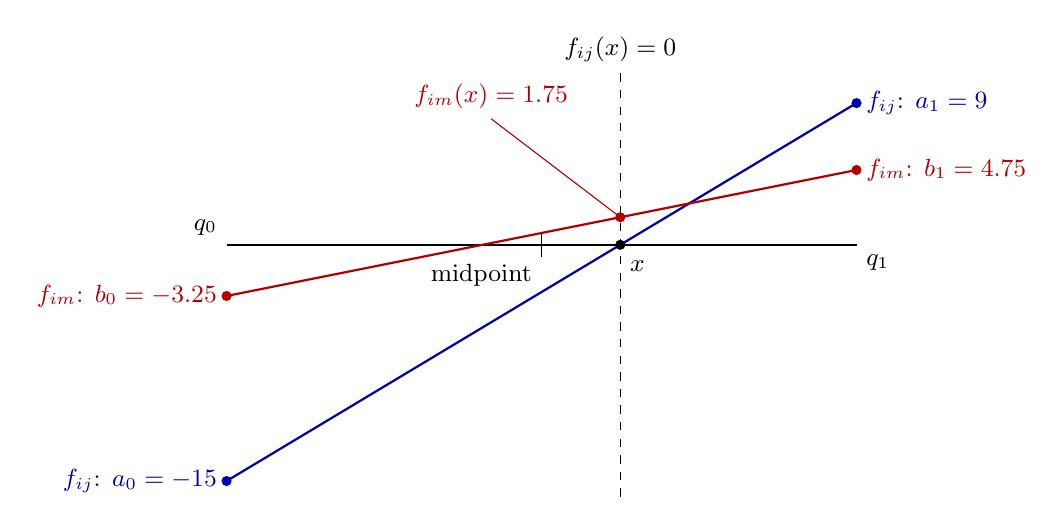
\begin{tikzpicture}[x=8cm, y=0.2cm, every node/.style={font=\small},
    pt/.style={circle, fill, inner sep=1.3pt}]
  \draw[thick] (0,0) -- (1,0);
  \node[above left] at (0,0) {$q_0$};
  \node[below right] at (1,0) {$q_1$};
  \draw (0.5,-0.8) -- (0.5,0.8);
  \node[below left] at (0.5,-0.6) {midpoint};
  \draw[blue!70!black, thick] (0,-15) -- (1,9);
  \draw[red!70!black, thick] (0,-3.25) -- (1,4.75);
  \node[pt, blue!70!black] at (0,-15) {};
  \node[left, blue!70!black] at (0,-15) {$f_{ij}$: $a_0 = -15$};
  \node[pt, blue!70!black] at (1,9) {};
  \node[right, blue!70!black] at (1,9) {$f_{ij}$: $a_1 = 9$};
  \node[pt, red!70!black] at (0,-3.25) {};
  \node[left, red!70!black] at (0,-3.25) {$f_{im}$: $b_0 = -3.25$};
  \node[pt, red!70!black] at (1,4.75) {};
  \node[right, red!70!black] at (1,4.75) {$f_{im}$: $b_1 = 4.75$};
  \draw[dashed] (0.625,-16) -- (0.625,11);
  \node[pt] at (0.625,0) {};
  \node[below right] at (0.625,-0.4) {$x$};
  \node[above] at (0.625,11) {$f_{ij}(x) = 0$};
  \node[pt, red!70!black] at (0.625,1.75) {};
  \draw[red!70!black, thin] (0.625,1.75) -- (0.42,8);
  \node[above, red!70!black] at (0.42,8) {$f_{im}(x) = 1.75$};
\end{tikzpicture}
\caption{The example of Step 4, along the edge from $q_0$ to $q_1$ (the horizontal axis is
$t$, from 0 at $q_0$ to 1 at $q_1$). Each $f$ is a straight line through its two corner values.
The vertex $x$ is where the blue line crosses zero, at $t = a_0/(a_0 - a_1) = 0.625$: not the
midpoint, in general. The red line's height there is $f_{im}(x)$, the answer.}
\label{fig:lemma}
\end{figure}

\subsection{Step 4: find the weights, then read off \texorpdfstring{$g(x)$}{g(x)}}

Name the corner values as \code{side2} does: $a_r = f_{ij}(q_r)$ for the bisector that defines
the vertex, $b_r = f_{im}(q_r)$ for the bisector being tested. By Step 3, the two conditions on
$x$ -- its weights sum to 1, and $f_{ij}(x) = 0$ -- are two \emph{linear} equations in the two
unknown weights:
\[
  \begin{aligned}
    \lambda_0 + \lambda_1 &= 1\\
    a_0\lambda_0 + a_1\lambda_1 &= 0
  \end{aligned}
  \qquad\text{that is}\qquad
  \underbrace{\begin{pmatrix} 1 & 1\\ a_0 & a_1 \end{pmatrix}}_{M}
  \begin{pmatrix} \lambda_0\\ \lambda_1 \end{pmatrix}
  = \begin{pmatrix} 1\\ 0 \end{pmatrix}.
\]
\emph{Cramer's rule} solves a square system $M\lambda = e$ whose determinant is not zero: each
unknown $\lambda_r$ is the determinant of $M$ with its column $r$ replaced by $e$, divided by
$\det M$. Here
\[
  \lambda_0 = \frac{\begin{vmatrix} 1 & 1\\ 0 & a_1 \end{vmatrix}}{\det M}
            = \frac{a_1}{a_1 - a_0},
  \qquad
  \lambda_1 = \frac{\begin{vmatrix} 1 & 1\\ a_0 & 0 \end{vmatrix}}{\det M}
            = \frac{-a_0}{a_1 - a_0},
  \qquad
  \det M = a_1 - a_0 .
\]
Now Step 3 once more, for $g$: substitute the two weights, then add the two fractions, which
share the denominator $a_1 - a_0$:
\begin{align*}
  g(x) &= b_0\lambda_0 + b_1\lambda_1
        = b_0\,\frac{a_1}{a_1 - a_0} + b_1\,\frac{-a_0}{a_1 - a_0}
        = \frac{b_0 a_1 - b_1 a_0}{a_1 - a_0}
        = \frac{\begin{vmatrix} b_0 & b_1\\ a_0 & a_1 \end{vmatrix}}
               {\begin{vmatrix} 1 & 1\\ a_0 & a_1 \end{vmatrix}} .
\end{align*}
The last step only recognises two $2\times2$ determinants, by the rule
$\begin{vsmallmatrix} p & q\\ r & s \end{vsmallmatrix} = ps - qr$: the top one is
$b_0a_1 - b_1a_0$, and the bottom one is $1\cdot a_1 - 1\cdot a_0 = a_1 - a_0 = \det M$.

\textbf{The numerator is $M$ with its row of ones replaced by $g$'s corner values}, although
Cramer's rule replaces \emph{columns}. (The \emph{cofactor} $C_{rc}$ of the entry in row $r$,
column $c$ is $(-1)^{r+c}$ times the determinant left when that row and that column are deleted;
for $M$, $C_{00} = +a_1$ and $C_{01} = -a_0$. Expanding a determinant along a row or a column
means summing each entry of it times its cofactor.) Both happen, at different moments:
\begin{itemize}
  \item \emph{Columns, one at a time, to get each weight.} For $\lambda_r$, column $r$ of $M$ is
    replaced by the right-hand side $(1, 0)$: a 1 at the top, 0 below. Expanding that determinant
    along the replaced column leaves a single term, 1 times the cofactor of its top entry, and a
    cofactor ignores its own row and column. So each Cramer numerator is the cofactor $C_{0r}$ of
    $M$'s \emph{top-row} entry in column $r$: here $C_{00} = a_1$ and $C_{01} = -a_0$, as above.
  \item \emph{The row, once, when the weights are combined.} Then
    $g(x) = b_0\lambda_0 + b_1\lambda_1 = (b_0 C_{00} + b_1 C_{01})/\det M$, and
    $b_0 C_{00} + b_1 C_{01}$ is exactly the expansion along its first row of a determinant whose
    first row is $(b_0, b_1)$. The cofactors $C_{00}$, $C_{01}$ do not involve the first row, so
    the other rows of that determinant are $M$'s: it is $\begin{vsmallmatrix} b_0 & b_1\\ a_0 & a_1
    \end{vsmallmatrix} = b_0a_1 - b_1a_0$.
\end{itemize}
It works out this way because the right-hand side is nonzero only in the top row, the row of
ones: that is what makes every Cramer numerator a cofactor of that one row.

\paragraph{Where $x$ falls.} With $x = (1-t)\,q_0 + t\,q_1$, the weights above give
$t = \lambda_1 = a_0/(a_0 - a_1)$: $x$ is where the straight line through $f_{ij}$'s two corner
values crosses zero. That is the midpoint only when $a_0 = -a_1$. If $a_0$ and $a_1$ have the same
sign, $t < 0$ or $t > 1$: $x$ is on the edge's line, but outside the edge. The formula holds there
too, since nothing above used $0 \le t \le 1$. A clipper, though, only creates a vertex on an edge
whose corner values $a_0$, $a_1$ have opposite signs, so the vertices it asks about have
$0 < t < 1$.

\paragraph{With numbers.} Take $p_i = (0,0,0)$, $p_j = (3,0,0)$, $p_m = (1, 0.5, 0)$, no weights,
and the edge from $q_0 = (-1,0,0)$ to $q_1 = (3,0,0)$. From the power distances,
$a_0 = 1 - 16 = -15$, $a_1 = 9 - 0 = 9$, $b_0 = 1 - 4.25 = -3.25$ and $b_1 = 9 - 4.25 = 4.75$.
Then $\det M = 24$, the weights are $\lambda = (\tfrac38, \tfrac58)$, so $t = 0.625$ and
$x = (1.5, 0, 0)$ -- on the bisector of $p_i$ and $p_j$, the plane of points whose first
coordinate is 1.5, and not at the edge's midpoint $(1, 0, 0)$. Then
\[
  f_{im}(x) = b_0\lambda_0 + b_1\lambda_1
            = (-3.25)\cdot\tfrac38 + (4.75)\cdot\tfrac58
            = \frac{(-3.25)(9) - (4.75)(-15)}{24} = \frac{42}{24} = 1.75 .
\]
Directly: $\pi_i(x) = 2.25$ and $\pi_m(x) = 0.25 + 0.25 = 0.5$, a difference of $1.75$. Positive:
$x$ is on $m$'s side. The predicate never divides; it takes $\sgn(42)\cdot\sgn(24) = +1$.

\paragraph{When $\det M = 0$.} Then $a_1 = a_0$: $f_{ij}$ has the same value at both ends, so it
is constant along the edge. Either it is never zero (the edge misses the bisector) or it is zero
everywhere (the edge lies in it). Either way there is no single vertex to ask about.

\subsection{The same pattern for \texorpdfstring{\code{side1}}{side1} and \texorpdfstring{\code{side3}}{side3}}

Nothing in Step 4 depended on the edge. A feature with $k+1$ corners gives $k+1$ weights; the
vertex needs $k$ bisector conditions to pin it down; with the sum condition that is a square
system of size $k+1$:

\begin{center}
\begin{tabularx}{\linewidth}{@{}l l l c L@{}}
\toprule
 & feature & conditions on the weights & $M$ & $f_{im}(x)$ \\
\midrule
\code{side1} & a corner $q_0$ & $\lambda_0 = 1$ & $1\times1$ & $f_{im}(q_0)$: no determinant \\
\code{side2} & an edge & sum 1, $f_{ij}(x) = 0$ & $2\times2$ & ratio of $2\times2$ determinants \\
\code{side3} & a triangle & sum 1, $f_{ij}(x) = 0$, $f_{ik}(x) = 0$ & $3\times3$ & ratio of
  $3\times3$ determinants \\
\bottomrule
\end{tabularx}
\end{center}
Each time, $M$'s first row is the row of ones (the sum condition), each further row holds one
defining bisector function's corner values, and the numerator is $M$ with its first row replaced
by $f_{im}$'s corner values. The lemma below is Steps 2 to 4 for any $k$, written once.

\subsection{The lemma in general}

\begin{lemma}[Cramer for affine functions]\label{lem:cramer}
Let $q_0, \dots, q_k$ be the corners of a domain feature ($k = 0, 1, 2$). Let
$h_1, \dots, h_k$ and $g$ be affine functions. Let $x$ be the point of the feature's affine
hull where $h_1(x) = \dots = h_k(x) = 0$. Write $h_s^{(r)} = h_s(q_r)$ and $g^{(r)} = g(q_r)$,
and let
\[
  M = \begin{pmatrix}
    1 & 1 & \cdots & 1 \\
    h_1^{(0)} & h_1^{(1)} & \cdots & h_1^{(k)} \\
    \vdots & & & \vdots \\
    h_k^{(0)} & h_k^{(1)} & \cdots & h_k^{(k)}
  \end{pmatrix}.
\]
If $\det M \neq 0$, then $x$ exists and is unique, and
\[
  g(x) = \frac{\det M_g}{\det M},
\]
where $M_g$ is $M$ with its first row (the row of ones) replaced by
$\bigl(g^{(0)}, \dots, g^{(k)}\bigr)$.
\end{lemma}

\begin{proof}
Write $x$ in barycentric coordinates, $x = \sum_r \lambda_r q_r$ with $\sum_r \lambda_r = 1$. By
\eqref{eq:affcomb}, $h_s(x) = \sum_r \lambda_r h_s^{(r)}$. So the conditions on $x$ are
\[
  \textstyle\sum_r \lambda_r = 1, \qquad \sum_r \lambda_r h_s^{(r)} = 0 \quad (s = 1..k),
\]
which is the square linear system $M\lambda = e_1$, where $e_1 = (1, 0, \dots, 0)^\mathsf{T}$.
If $\det M \neq 0$ it has exactly one solution. By Cramer's rule,
\[
  \lambda_r = \frac{\det M^{[r]}}{\det M},
\]
where $M^{[r]}$ is $M$ with column $r$ replaced by $e_1$. Expanding $\det M^{[r]}$ along that
column leaves only its top entry, so $\det M^{[r]} = C_{0r}$, the cofactor of the entry in row 0,
column $r$ of $M$. Then, by \eqref{eq:affcomb} again,
\[
  g(x) = \sum_r \lambda_r g^{(r)} = \frac{\sum_r g^{(r)} C_{0r}}{\det M}.
\]
The numerator is the expansion along row 0 of a determinant whose row 0 is
$(g^{(0)}, \dots, g^{(k)})$ and whose other rows are those of $M$, which is $\det M_g$. The
cofactors $C_{0r}$ do not involve row 0, so changing it does not change them.
\end{proof}

\paragraph{What it means for the predicates.} Take $h_s$ to be the bisector functions that
define the vertex ($f_{ij}$, and $f_{ik}$ for a face) and $g = f_{im}$. Then
\[
  \sgn f_{im}(x) = \sgn(\det M_g)\cdot\sgn(\det M).
\]
Both determinants are polynomials in $f$ values at the corners, so they are polynomials in the
input. That is the whole trick. Three remarks:
\begin{itemize}
  \item \textbf{The denominator's sign is not fixed.} Listing the corners in another order permutes
    the columns of $M$ and $M_g$ together. Both determinants can flip sign, and their ratio
    cannot. So the predicate must multiply the two signs: it cannot assume $\det M > 0$.
  \item \textbf{$\det M = 0$ means the equations do not define a unique vertex}: they have no
    solution, or infinitely many. No solution when the feature is parallel to a bisector it does
    not lie in; infinitely many when it lies in that bisector, or the bisectors meet it in a line
    instead of a point; and the feature itself may be degenerate (coincident or collinear corners),
    or two seeds coincide (\secref{sec:f}). The clipper never asks about such a vertex, because it
    never creates one. The oracle detects exactly the same cases: its linear system has
    determinant $\det M$, as \secref{ssec:dexpl} shows for \code{side2}.
  \item \textbf{$x$ does not have to lie inside the feature.} The lemma works on the whole line or
    plane through it, and some $\lambda_r$ may be negative. The predicate does not care. The tests
    use random features whose vertex is often outside them.
\end{itemize}

% ======================================================================================
\section{\texorpdfstring{\code{side1}}{side1}: a domain corner}\label{sec:side1}

The case $k = 0$ of the lemma: $M = (1)$ and $M_g = (g^{(0)})$, so
\[
  f_{im}(x) = f_{im}(q).
\]
The vertex is the corner $q$ itself, nothing needs solving, and the predicate is the sign of one
$f$ value, in the difference form~\eqref{eq:diffform}. Degree 2.

\paragraph{Worked example} (from \code{test\_side1.cpp}). $p_i = 0$, $p_m = (2,0,0)$, no
weights, $q = (\tfrac12, 0, 0)$. Then $p_m - p_i = (2,0,0)$ and
$(q - p_i) + (q - p_m) = (\tfrac12,0,0) + (-\tfrac32,0,0) = (-1,0,0)$, so $f_{im}(q) = -2$:
answer $-1$. Directly: $\pi_i(q) = \tfrac14$ and $\pi_m(q) = \tfrac94$, a difference of $-2$.

\paragraph{Symmetry.} $f_{mi} = -f_{im}$, so swapping $i$ and $m$ flips the sign. The test
checks this on 50\,000 inputs.

% ======================================================================================
\section{\texorpdfstring{\code{side2}}{side2}: an edge crossing one bisector}\label{sec:side2}

\begin{figure}[ht]
\centering
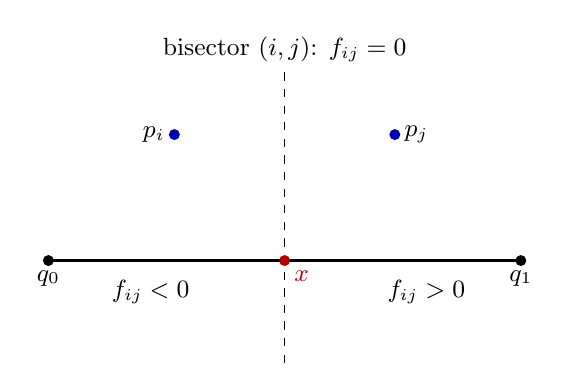
\begin{tikzpicture}[scale=1.0, every node/.style={font=\small},
    pt/.style={circle, fill, inner sep=1.4pt}]
  \coordinate (q0) at (-1,0);
  \coordinate (q1) at (5,0);
  \coordinate (pi) at (0.6,1.6);
  \coordinate (pj) at (3.4,1.6);
  \coordinate (x)  at (2,0);
  \draw[thick] (q0) -- (q1);
  \draw[dashed] (2,-1.3) -- (2,2.4) node[above] {bisector $(i,j)$: $f_{ij} = 0$};
  \node[pt] at (q0) {}; \node[below] at (q0) {$q_0$};
  \node[pt] at (q1) {}; \node[below] at (q1) {$q_1$};
  \node[pt, red!70!black] at (x) {}; \node[below right, red!70!black] at (x) {$x$};
  \node[pt, blue!70!black] at (pi) {}; \node[left] at (pi) {$p_i$};
  \node[pt, blue!70!black] at (pj) {}; \node[right] at (pj) {$p_j$};
  \node at (0.3,-0.4) {$f_{ij} < 0$};
  \node at (3.8,-0.4) {$f_{ij} > 0$};
\end{tikzpicture}
\caption{An E vertex: where the domain edge $q_0q_1$ crosses the bisector of $i$ and $j$.
\code{side2} asks on which side of a \emph{third} bisector, $(i,m)$, it lies.}
\label{fig:side2}
\end{figure}

\paragraph{Signature} (fixed by the test):
\code{side2(pi, wi, pj, wj, pm, wm, q0, q1)}.

\subsection{Derivation}

Name the four $f$ values at the corners:
\begin{align*}
  a_0 &= f_{ij}(q_0), & a_1 &= f_{ij}(q_1) && \text{(the bisector that defines $x$)},\\
  b_0 &= f_{im}(q_0), & b_1 &= f_{im}(q_1) && \text{(the bisector tested)}.
\end{align*}

\emph{Directly.} Write $x = (1-t)\,q_0 + t\,q_1$. Then $f_{ij}(x) = (1-t)a_0 + t a_1 = 0$ gives
$t = a_0/(a_0 - a_1)$, and
\[
  f_{im}(x) = (1-t)\,b_0 + t\,b_1 = \frac{b_0(a_0 - a_1) - a_0 b_0 + a_0 b_1}{a_0 - a_1}
            = \frac{a_0 b_1 - a_1 b_0}{a_0 - a_1}.
\]

\emph{By the lemma}, with $k = 1$, $h_1 = f_{ij}$, $g = f_{im}$:
\begin{equation}\label{eq:side2}
  f_{im}(x) =
  \frac{\begin{vmatrix} b_0 & b_1 \\ a_0 & a_1 \end{vmatrix}}
       {\begin{vmatrix} 1 & 1 \\ a_0 & a_1 \end{vmatrix}}
  = \frac{b_0 a_1 - b_1 a_0}{a_1 - a_0}.
\end{equation}
It is the same expression: multiply the top and bottom of the direct one by $-1$.

\keybox{\centering $\sgn f_{im}(x) = \sgn(N)\cdot\sgn(D)$, \quad
  $N = b_0 a_1 - b_1 a_0$ (degree 4), \quad $D = a_1 - a_0$ (degree 2).}

\noindent
Cost: four $f$ evaluations, one $2\times2$ determinant, one difference.

\subsection{The denominator, explained}\label{ssec:dexpl}

By~\eqref{eq:affine}, $a_1 - a_0 = f_{ij}(q_1) - f_{ij}(q_0) = 2\,(q_1 - q_0)\cdot(p_j - p_i)$:
the constants cancel. So $D = 0$ exactly when the edge is perpendicular to $p_j - p_i$, which
means parallel to the bisector (or $p_j = p_i$). Then there is no single crossing: none if the
edge's line misses the bisector, a whole line of them if it lies inside it. This is also exactly the single
coefficient of the oracle's $1\times1$ system: the same quantity, written differently.

This also gives an alternative way to compute $D$, straight from coordinates. Its value is
identical. In \code{Bounded} its error bound is smaller, because it is one dot product of
differences rather than a difference of two degree-2 results. That is optional and only worth it
if the filter rate disappoints. If you use it, keep its sign consistent with $N$'s. Both forms
above are $a_1 - a_0$, not $a_0 - a_1$.

\subsection{Worked example}
The same numbers as the hand-written test in \code{test\_side2.cpp}.

$p_i = 0$, $p_j = (2,0,0)$, edge $q_0 = (-1,0,0)$ to $q_1 = (3,0,0)$, $p_m = (5,0,0)$, no
weights. With $p_i = 0$, $f_{ia}(q) = 2\,q\cdot p_a - \norm{p_a}^2$:
\begin{align*}
  f_{ij}(q) &= 4q_x - 4: & a_0 &= -8, & a_1 &= 8,\\
  f_{im}(q) &= 10q_x - 25: & b_0 &= -35, & b_1 &= 5.
\end{align*}
$N = (-35)(8) - (5)(-8) = -240$ and $D = 8 - (-8) = 16$, so $f_{im}(x) = -15$: answer $-1$.

Check: the crossing is $x = (1,0,0)$, with $\pi_i(x) = 1$ and $\pi_m(x) = 16$, a difference of
$-15$. The direct alternative for $D$ gives $2\,(4,0,0)\cdot(2,0,0) = 16$. \checkmark

\subsection{Symmetries the tests check}

\begin{itemize}
  \item \textbf{The edge read backwards.} Swapping $q_0$ and $q_1$ swaps $a_0 \leftrightarrow a_1$
    and $b_0 \leftrightarrow b_1$. That negates $N$ and negates $D$, so the ratio is unchanged.
    This is the reason for multiplying the two signs.
  \item \textbf{$i$ and $j$ exchanged.} The vertex is the same point, where $f_{ji} = -f_{ij} = 0$.
    And $f_{jm} = \pi_j - \pi_m = f_{im} - f_{ij}$, which equals $f_{im}$ at $x$. Same answer.
\end{itemize}

% ======================================================================================
\section{\texorpdfstring{\code{side3}}{side3}: a triangle crossing two bisectors}\label{sec:side3}

\begin{figure}[ht]
\centering
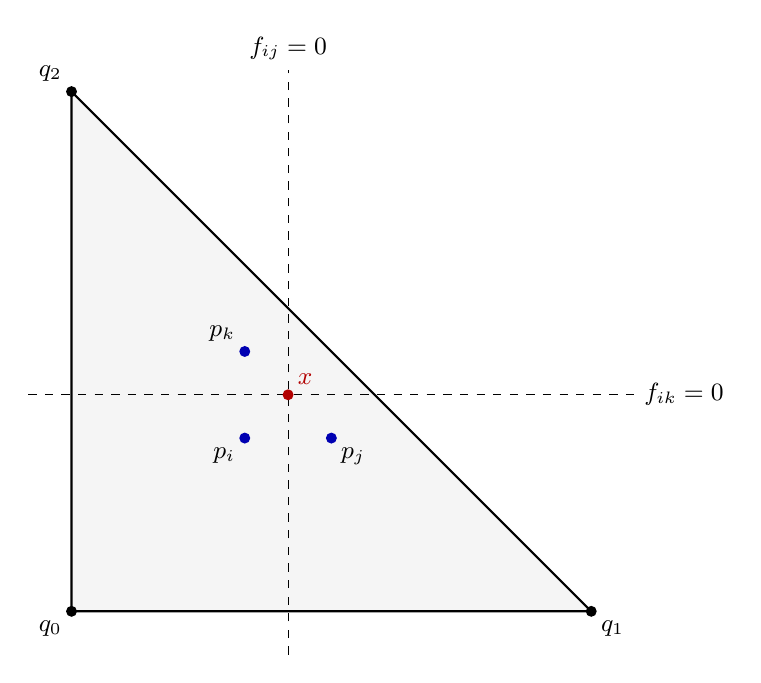
\begin{tikzpicture}[scale=0.55, every node/.style={font=\small},
    pt/.style={circle, fill, inner sep=1.4pt}]
  \coordinate (q0) at (-4,-4);
  \coordinate (q1) at (8,-4);
  \coordinate (q2) at (-4,8);
  \fill[gray!8] (q0) -- (q1) -- (q2) -- cycle;
  \draw[thick] (q0) -- (q1) -- (q2) -- cycle;
  \draw[dashed] (1,-5) -- (1,8.5) node[above] {$f_{ij} = 0$};
  \draw[dashed] (-5,1) -- (9,1) node[right] {$f_{ik} = 0$};
  \node[pt] at (q0) {}; \node[below left] at (q0) {$q_0$};
  \node[pt] at (q1) {}; \node[below right] at (q1) {$q_1$};
  \node[pt] at (q2) {}; \node[above left] at (q2) {$q_2$};
  \node[pt, red!70!black] at (1,1) {}; \node[above right, red!70!black] at (1,1) {$x$};
  \node[pt, blue!70!black] at (0,0) {}; \node[below left] at (0,0) {$p_i$};
  \node[pt, blue!70!black] at (2,0) {}; \node[below right] at (2,0) {$p_j$};
  \node[pt, blue!70!black] at (0,2) {}; \node[above left] at (0,2) {$p_k$};
\end{tikzpicture}
\caption{An F vertex: where the plane of the triangle meets two bisectors at once. Drawn in the
triangle's plane, with the numbers of the worked example (\secref{ssec:side3ex}).}
\label{fig:side3}
\end{figure}

\paragraph{Signature:} \code{side3(pi, wi, pj, wj, pk, wk, pm, wm, q0, q1, q2)}.

\subsection{Derivation}

Nine $f$ values, three per corner $q_r$:
\[
  a_r = f_{ij}(q_r), \qquad c_r = f_{ik}(q_r), \qquad b_r = f_{im}(q_r), \qquad r = 0, 1, 2.
\]
The lemma with $k = 2$, $h_1 = f_{ij}$, $h_2 = f_{ik}$, $g = f_{im}$:
\begin{equation}\label{eq:side3}
  f_{im}(x) =
  \frac{\begin{vmatrix} b_0 & b_1 & b_2 \\ a_0 & a_1 & a_2 \\ c_0 & c_1 & c_2 \end{vmatrix}}
       {\begin{vmatrix} 1 & 1 & 1 \\ a_0 & a_1 & a_2 \\ c_0 & c_1 & c_2 \end{vmatrix}}.
\end{equation}

\keybox{\centering $\sgn f_{im}(x) = \sgn(N)\cdot\sgn(D)$, \quad
  $N$ of degree 6, \quad $D$ of degree 4.}

\subsection{Structure: share the bottom rows}

Both determinants have the same bottom two rows. Expand both along the top row. The cofactors are
the same three $2\times2$ minors of the $a$ and $c$ rows:
\[
  \mu_0 = a_1c_2 - a_2c_1, \qquad \mu_1 = a_0c_2 - a_2c_0, \qquad \mu_2 = a_0c_1 - a_1c_0,
\]
and then
\begin{equation}\label{eq:side3mu}
  N = b_0\,\mu_0 - b_1\,\mu_1 + b_2\,\mu_2, \qquad D = \mu_0 - \mu_1 + \mu_2 .
\end{equation}
So the predicate costs nine $f$ values, three minors (six products), and two cheap
combinations. In the exact path this matters: the minors are the expensive products, and this
way they are computed once instead of twice.

\paragraph{An alternative denominator.} Subtract column 0 from columns 1 and 2 of $D$. The
determinant is unchanged, and the row of ones becomes $(1, 0, 0)$:
\[
  D = (a_1 - a_0)(c_2 - c_0) - (a_2 - a_0)(c_1 - c_0).
\]
As in \code{side2}, each difference is a dot product of coordinate differences, for example
$a_r - a_0 = 2\,(q_r - q_0)\cdot(p_j - p_i)$. That is exactly the oracle's $2\times2$ system
matrix, so $D$ is its determinant. Same value, tighter error bound, optional.

\subsection{Worked example}\label{ssec:side3ex}
The same numbers as the hand-written test in \code{test\_side3.cpp}.

$p_i = 0$, $p_j = (2,0,0)$, $p_k = (0,2,0)$, $p_m = (1,1,2)$, no weights, triangle
$q_0 = (-4,-4,0)$, $q_1 = (8,-4,0)$, $q_2 = (-4,8,0)$ (figure~\ref{fig:side3}). With
$f_{ia}(q) = 2q\cdot p_a - \norm{p_a}^2$:
\begin{align*}
  f_{ij}(q) &= 4q_x - 4: & a &= (-20,\ 28,\ -20),\\
  f_{ik}(q) &= 4q_y - 4: & c &= (-20,\ -20,\ 28),\\
  f_{im}(q) &= 2(q_x + q_y + 2q_z) - 6: & b &= (-22,\ 2,\ 2).
\end{align*}
The minors: $\mu_0 = 28\cdot28 - (-20)(-20) = 384$,
$\mu_1 = (-20)(28) - (-20)(-20) = -960$, and $\mu_2 = (-20)(-20) - (28)(-20) = 960$. So
\[
  D = 384 + 960 + 960 = 2304, \qquad N = (-22)(384) - 2(-960) + 2(960) = -4608,
\]
and $f_{im}(x) = -2$: answer $-1$. The alternative gives $D = 48\cdot48 - 0\cdot0 = 2304$.

Check: the vertex is $x = (1,1,0)$, with $\pi_i(x) = 2$ and $\pi_m(x) = 0 + 0 + 4 = 4$, a
difference of $-2$. \checkmark

\subsection{Symmetries the tests check}

\begin{itemize}
  \item \textbf{Any order of the corners.} A permutation of the corners permutes the columns of both
    determinants in the same way, so both are multiplied by the same $\pm1$.
  \item \textbf{Any of $i, j, k$ called $i$.} The vertex is the point where all three power
    distances are equal, so $f_{im}(x) = f_{jm}(x) = f_{km}(x)$. The test rotates $(i,j,k)$ and
    swaps $j$ and $k$. This is a real check of the implementation, not of the formula: all nine
    $f$ values change.
\end{itemize}

\subsection{Cost of the exact path}

This is the most expensive predicate: degree 6, with expansions of the $f$ values multiplied
three deep. The product of two \code{DynamicExpansion}s compresses its result, which keeps each
level short. Without that, every level would be slower than the one before. Only near-degenerate
inputs reach this path. The filter decides the rest.

% ======================================================================================
\section{\texorpdfstring{\code{side4}}{side4}: a Voronoi vertex}\label{sec:side4}

\paragraph{Signature:} \code{side4(pi, wi, pj, wj, pk, wk, pl, wl, pm, wm)}.

The vertex $x$ has equal power distance to $i$, $j$, $k$ and $l$. In three dimensions it is the
centre of the power sphere through the four seeds. There is no domain feature, so the lemma does
not apply. Instead the three bisector equations are solved directly, and the solution is
substituted, again without ever being computed.

\subsection{Work relative to \texorpdfstring{$p_i$}{p\_i}}

Put the origin at $p_i$. Let $d_a = p_a - p_i$ and $x' = x - p_i$. Then
\[
  f_{ia}(x) = \norm{x'}^2 - w_i - \norm{x' - d_a}^2 + w_a = 2\,x'\cdot d_a - c_a,
  \qquad
  \boxed{c_a = \norm{d_a}^2 + w_i - w_a.}
\]
Compare with~\eqref{eq:affine}: the large, cancelling $\norm{p_a}^2 - \norm{p_i}^2$ has become
$\norm{d_a}^2$, a square of differences. Everything below is built from the $d_a$ and the
$c_a$, so it is translation-invariant, for the same reasons as~\eqref{eq:diffform}.

\subsection{Derivation}

The vertex satisfies $f_{ia}(x) = 0$ for $a = j, k, l$, that is
\[
  2\,d_a\cdot x' = c_a, \qquad a = j, k, l.
\]
Consider the $4\times4$ determinant whose rows are $(2d_a,\ c_a)$ for $a = j, k, l, m$. From
the last column, subtract $x'_1$ times column 1, $x'_2$ times column 2 and $x'_3$ times
column 3. This does not change the determinant. Each last entry becomes
$c_a - 2d_a\cdot x' = -f_{ia}(x)$, which is $0$ for $a = j, k, l$ and $-f_{im}(x)$ for $a = m$:
\[
  \begin{vmatrix} 2d_j & c_j \\ 2d_k & c_k \\ 2d_l & c_l \\ 2d_m & c_m \end{vmatrix}
  =
  \begin{vmatrix} 2d_j & 0 \\ 2d_k & 0 \\ 2d_l & 0 \\ 2d_m & -f_{im}(x) \end{vmatrix}
  = -f_{im}(x)\,\begin{vmatrix} 2d_j \\ 2d_k \\ 2d_l \end{vmatrix},
\]
expanding along the last column, whose only non-zero entry sits at position $(4,4)$ with
cofactor sign $+$. Each $d_a$ is a row of three numbers. Now drop the 2s. Factoring 2 out of
each of the first three columns gives $2^3$ on both sides, which cancels \emph{exactly}, not
just in sign:
\begin{equation}\label{eq:side4}
  f_{im}(x) = -\,\frac{\begin{vmatrix} d_j & c_j \\ d_k & c_k \\ d_l & c_l \\ d_m & c_m \end{vmatrix}}
                      {\begin{vmatrix} d_j \\ d_k \\ d_l \end{vmatrix}} .
\end{equation}

\keybox{\centering $\sgn f_{im}(x) = -\,\sgn(N)\cdot\sgn(D)$, \quad
  $N = \det_4$ (degree 5), \quad $D = \det_3$ (degree 3). \quad \textbf{Mind the minus.}}

\noindent
Degrees: three columns of $d$ entries (degree 1) and one column of $c$ entries (degree 2) make
$N$ degree $1+1+1+2 = 5$. $D$ is degree 3.

\subsection{Structure: four triple products}

Write $T(a,b,c) = \det[d_a; d_b; d_c] = d_a\cdot(d_b\times d_c)$, the triple product. Expand
$N$ along its last column. The cofactor signs for rows $1..4$ of column 4 are $-, +, -, +$:
\begin{equation}\label{eq:side4exp}
  N = -\,c_j\,T(k,l,m) + c_k\,T(j,l,m) - c_l\,T(j,k,m) + c_m\,T(j,k,l), \qquad D = T(j,k,l).
\end{equation}
So the predicate is four $c$ values and four triple products, one of which is $D$ itself. Get
one cofactor sign wrong and the answer is wrong only on \emph{some} inputs. The hand-worked
tests and the permutation test are what catch that.

\subsection{The \texorpdfstring{\code{orient3d}}{orient3d} trap}

$T$ has the same shape as \code{orient3d\_det}, so reusing it is tempting. But \code{orient3d}
follows mesh-dev's convention, not this formula's:
\begin{align*}
  \code{orient3d}(a,b,c,d) &= (a-d)\cdot\bigl((c-d)\times(b-d)\bigr),\\
  \text{so}\quad \code{orient3d}(p_j, p_k, p_l, p_i) &= d_j\cdot(d_l\times d_k) = -\,T(j,k,l).
\end{align*}
Reusing it is fine if the sign is accounted for. Writing $T$ directly is three lines and has no
trap.

\subsection{Worked example}
The same numbers as the hand-written test in \code{test\_side4.cpp}.

$p_i = 0$, $p_j = (2,0,0)$, $p_k = (0,2,0)$, $p_l = (0,0,2)$, $p_m = (3,3,3)$, no weights. Then
$d_a = p_a$, $c_j = c_k = c_l = 4$ and $c_m = 27$. The triple products:
\begin{align*}
  T(j,k,l) &= (2,0,0)\cdot\bigl((0,2,0)\times(0,0,2)\bigr) = (2,0,0)\cdot(4,0,0) = 8,\\
  T(k,l,m) &= (0,2,0)\cdot\bigl((0,0,2)\times(3,3,3)\bigr) = (0,2,0)\cdot(-6,6,0) = 12,\\
  T(j,l,m) &= (2,0,0)\cdot(-6,6,0) = -12,\\
  T(j,k,m) &= (2,0,0)\cdot\bigl((0,2,0)\times(3,3,3)\bigr) = (2,0,0)\cdot(6,0,-6) = 12.
\end{align*}
By~\eqref{eq:side4exp}, $N = -4\cdot12 + 4\cdot(-12) - 4\cdot12 + 27\cdot8 = 72$, $D = 8$, and
$f_{im}(x) = -72/8 = -9$: answer $-1$.

Check: the vertex is $x = (1,1,1)$, with $\pi_i(x) = 3$ and $\pi_m(x) = 4+4+4 = 12$, a
difference of $-9$. \checkmark\ The same test then gives $p_m$ a weight of 10. Only $c_m$ changes,
to $27 - 10 = 17$, so $N = -144 + 136 = -8$ and $f_{im}(x) = +1$: the weight pulls the vertex to
$m$'s side.

\subsection{Symmetries the tests check}

All 24 orders of $(i,j,k,l)$ must give the same sign, since the vertex and its power distance are
the same. Permuting $j, k, l$ among themselves permutes rows of both determinants together, so
it is easy. Exchanging $i$ with one of them changes \emph{every} $d_a$ and $c_a$. That this still
gives the same sign is true of the mathematics, and it is the strongest check there is of the
sign bookkeeping in~\eqref{eq:side4} and~\eqref{eq:side4exp}.

% ======================================================================================
\section{Evaluating them: fast when easy, exact when not}\label{sec:eval}

Every predicate has the same skeleton as \code{orient2d}, \code{orient3d} and \code{side1}.

\subsection{One formula, several number types}

Write each formula (the $f$ values, the minors, the triple products, $N$ and $D$) once, as a
template over a number type $T$. The same text then means three things:

\begin{center}
\begin{tabularx}{\linewidth}{@{}l L@{}}
\toprule
$T$ & what the formula computes \\
\midrule
\code{double} & a rounded value: fast, and wrong exactly where it matters \\
\code{Bounded} & a rounded value \emph{and} a certified bound on its error: the filter \\
\code{DynamicExpansion} & the exact value, as a list of non-overlapping doubles: the exact path \\
\bottomrule
\end{tabularx}
\end{center}

\subsection{The filter}

A \code{Bounded} carries a value $v$ and an error $e$ with $|v - \text{exact}| \le e$. Inputs
have $e = 0$. With $u = 2^{-53}$, each operation propagates the bound:
\[
  a \pm b:\ e = e_a + e_b + u|v|, \qquad
  a\cdot b:\ e = |a|\,e_b + |b|\,e_a + e_a e_b + u|v|, \qquad
  -a:\ e = e_a,
\]
inflated by $1 + 2^{-48}$ to cover the rounding of the bound itself. At the end,
\code{certain\_sign} says:
\begin{itemize}
  \item $|v| > e$: the sign of $v$ is the true sign;
  \item $v = 0$ and $e = 0$: the value is exactly zero;
  \item otherwise: don't know.
\end{itemize}
The filter can be unsure. It cannot be wrong. Because the bound is built by the operators, it is
sound for any formula, including these new ones, with no hand derivation of error constants.

\subsection{The decision}

\begin{enumerate}
  \item Evaluate $N$ and $D$ with \code{Bounded}.
  \item If \code{certain\_sign} says $N$ is certainly 0, the answer is 0 whatever $D$ is: $D \neq 0$
    is the precondition, so $D$'s sign is not needed. Count one \code{filtered} call. (This is
    what the code does; it does not certify $D$ first.)
  \item Otherwise, if \code{certain\_sign} decides \emph{both}, the answer is the product of the
    two signs. Count one \code{filtered} call.
  \item Otherwise, evaluate $N$ and $D$ exactly with \code{DynamicExpansion}, take the sign of each
    (the sign of the largest component), and return their product. Count one \code{exact} call.
\end{enumerate}
\noindent\textbf{The \code{side4} minus.} In this document \code{side4}'s $N$ is $\det_4$ itself,
so its answer is $-\sgn N\cdot\sgn D$. The code folds the minus into the numerator instead:
\code{side4\_terms} returns $\{-\det_4,\ \det_3\}$, and the decision above, with no extra minus,
is then the same for all four predicates.

Two refinements are possible later, and neither is needed for correctness. If the filter
certified $D$ but not $N$, only $N$ needs the exact path. And the $f$ values could be computed
once and shared between $N$ and $D$, which the minor structure of \code{side3} already does.

\paragraph{Why both signs.} It is tempting to certify only $N$ and assume $D > 0$. As shown in
\secref{sec:lemma}, the sign of $D$ depends on the order of the corners (or, for \code{side4},
on the orientation of $p_i, p_j, p_k, p_l$), which is arbitrary. So it is part of the answer.

\paragraph{The precondition.} $D \neq 0$. If the exact $D$ is zero, the caller asked about a
vertex its equations do not define uniquely. That is a bug in the caller, and an assertion should say so. The
tests keep assertions on in every build type.

\subsection{Why \texorpdfstring{\code{DynamicExpansion}}{DynamicExpansion}}

\code{Expansion<N>} carries a worst-case capacity in its type. A sum of $M$ and $N$ components
needs $M+N$, and a product needs $2MN$. That works for \code{orient3d} (192 components, 1.5\,KB),
but the bounds multiply with the degree. \code{side2} would need about ten thousand components,
and \code{side3} millions, far more than a stack holds. Those are worst cases. The real length of
an expansion depends on how many bits the value actually has, which is usually far fewer, and
known only once the value is computed. \code{DynamicExpansion} keeps its first 32 components
inline and moves to the heap beyond that. An exact evaluation therefore avoids the heap only if
\emph{every intermediate value} stays within 32 components, not merely the final result:
products and the merge in a sum can be longer than what is left at the end.

\subsection{Counters}

Each predicate has its own thread-local \code{PredicateCounts}: \code{side2\_counts()},
\code{side3\_counts()} and \code{side4\_counts()}, like \code{side1\_counts()}. Every call
increments exactly one of \code{filtered} and \code{exact}. The tests check that the two add up
to the number of calls, and they use the ratio to check that the filter does its job.

% ======================================================================================
\section{How they are tested}\label{sec:tests}

\subsection{The oracle}

The oracle (\code{tests/side\_support.h}) shares no formula with the predicates. It builds the
vertex's defining linear system (the bisector equations, in barycentric or Cartesian unknowns),
solves it exactly in GMP rationals by Gaussian elimination, and compares $\pi_i(x)$ with
$\pi_m(x)$ straight from the definition $\norm{x - p}^2 - w$. It returns ``no vertex'' when the
system is singular, and the tests then skip the case. Two derivations from different starting
points that agree on hundreds of thousands of inputs is the evidence.

\subsection{The input families}

\begin{center}
\begin{tabularx}{\linewidth}{@{}l L@{}}
\toprule
family & what it is for \\
\midrule
random & coordinates with random signs, full significands and exponents in $[-20, 20]$, half the
  seeds weighted. Cancellation at every scale. The filter should decide nearly all of them \\
lattice & small integers in $[-2,2]$. Ties are common, and the answer must then be exactly 0 \\
far lattice & the same, moved by $2^{20}$ and by $10^6 + 0.5$. Same answers, ties included,
  under heavy cancellation \\
nudged ties & a lattice tie with one non-zero coordinate moved by one ulp. Tiny non-zero
  answers. They must mostly reach the exact path, and constructing the vertex in doubles must get
  some of them wrong (otherwise the test would be too easy) \\
\bottomrule
\end{tabularx}
\end{center}

\subsection{Thresholds}

The required values are the suites' thresholds. They were set on 1 October 2026 below what a
throwaway reference implementation reached (with a different random seed, whose results were not
kept). The ``measured'' values are those of the actual \code{side.h}, on 5 October 2026, on the
suites' own input families and seeds, from \code{build/rvd-measure-side}
(\code{tests/measure\_side.cpp}; setup and timings in \code{documents/arithmetic}, section 9).
They are deterministic, so running the program again reproduces them exactly.

\begin{center}
\begin{tabular}{@{}lcccc@{}}
\toprule
 & filter on random & lattice ties & nudged reaching exact & doubles wrong \\
 & (required / measured) & (measured) & (required / measured) & (measured) \\
\midrule
\code{side1} & 99\% / 100.00\% & 4.54\% & 80\% / 88.1\% & 76.3\% \\
\code{side2} & 99\% / 100.00\% & 3.26\% & 80\% / 91.6\% & 71.8\% \\
\code{side3} & 95\% / 98.19\%  & 2.77\% & 80\% / 91.6\% & 67.7\% \\
\code{side4} & 99\% / 99.99\%  & 3.98\% & 80\% / 93.6\% & 65.2\% \\
\bottomrule
\end{tabular}
\end{center}

\noindent
Not every nudged tie needs the exact path. A nudge can move a value far enough from zero,
relative to its error bound, for the filter to certify it. ``Doubles wrong'' is the share of
nudged ties on which constructing the vertex in doubles, then comparing the two power distances,
gets the sign wrong; the suites only require it to be above zero.

% ======================================================================================
\section{A preview: ties}\label{sec:ties}

For now an exact tie returns 0, and the lattice tests expect that. A later step replaces 0 with
\emph{symbolic perturbation} (DESIGN.tex, section 6.4). The idea, so that it is not a surprise:
imagine every weight increased by an infinitesimal $\varepsilon_a$, with
$\varepsilon_0 \gg \varepsilon_1 \gg \varepsilon_2 \gg \cdots$. Increasing $w_a$ by
$\varepsilon_a$ lowers $\pi_a$ by $\varepsilon_a$, so it shifts
\[
  f_{ia} \;\longmapsto\; f_{ia} + (\varepsilon_a - \varepsilon_i).
\]
Every $f$ value moves by a constant, so the perturbed $N$ is the true $N$ plus terms in the
$\varepsilon$s, whose coefficients are smaller determinants of the same family, with a row
replaced by ones. When the true value is 0, the sign is that of the first non-zero coefficient,
in order of priority. For \code{side1} this is simple: $f_{im}(q) = 0$ becomes
$\varepsilon_m - \varepsilon_i$, whose sign is decided by which index is smaller. For the others
the chain always ends at the vertex's own $D$, which is non-zero by the precondition. The details
are worked out in \code{documents/arithmetic/arithmetic.tex}, section 8. Nothing in this document's formulas changes, but the
formulas will be reused for the coefficients, which is one more reason to write them cleanly.

% ======================================================================================
\section{Checklist}\label{sec:checklist}

\begin{itemize}
  \item $f$ values in the difference form~\eqref{eq:diffform}, through \code{bisector\_value}.
  \item The answer is $\sgn N\cdot\sgn D$, never $\sgn N$ alone. \code{side4} has an extra minus.
  \item \code{side2}: $N = b_0a_1 - b_1a_0$, $D = a_1 - a_0$. Both or neither negated.
  \item \code{side3}: three minors $\mu_r$, shared by $N$ and $D$; cofactor signs $+,-,+$.
  \item \code{side4}: coordinates relative to $p_i$; $c_a = \norm{d_a}^2 + w_i - w_a$; cofactor
    signs $-,+,-,+$ on the column of $c$s; \code{orient3d} is $-T$.
  \item Filter: an answer needs both $N$ and $D$ certain, or $N$ certainly zero (then the answer is
    0, by the precondition $D \neq 0$).
  \item One counter increment per call, in the right counter.
  \item Assert $D \neq 0$ on the exact path.
  \item A suite joins the build as soon as \code{sideK(} appears in \code{side.h}. From then on it
    has to compile and pass.
  \item Run one suite with \code{cmake --build build \&\& build/rvd-tests-side2}.
\end{itemize}

\subsection*{Summary}

\begin{center}
\begin{tabularx}{\linewidth}{@{}l L L c c@{}}
\toprule
 & numerator $N$ & denominator $D$ & deg $N$ & deg $D$ \\
\midrule
\code{side1} & $f_{im}(q)$ & $1$ & 2 & 0 \\
\code{side2} & $b_0a_1 - b_1a_0$ & $a_1 - a_0$ & 4 & 2 \\
\code{side3} & $b_0\mu_0 - b_1\mu_1 + b_2\mu_2$ & $\mu_0 - \mu_1 + \mu_2$ & 6 & 4 \\
\code{side4} & $\det_4[(d_a, c_a)]_{a=j,k,l,m}$, answer negated & $T(j,k,l)$ & 5 & 3 \\
\bottomrule
\end{tabularx}
\end{center}

\end{document}
